% % !TEX program = pdflatex
% \documentclass{beamer}

% % \usetheme{Madrid}
% \usepackage{amsmath,mathrsfs}
% \usepackage{tikz}

\tikzset{elegant/.style={smooth,thick,samples=50,cyan}}
\tikzset{eaxis/.style={->,>=stealth}}

% \begin{document}
\begin{frame}
    \frametitle{Wasserstein Distance}
    \resizebox{\textwidth}{!}{
    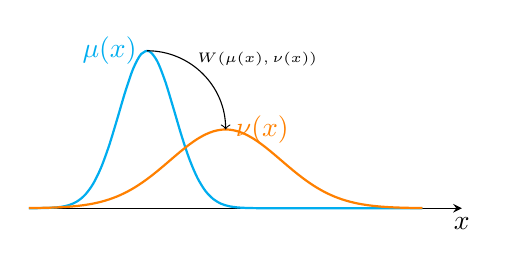
\begin{tikzpicture}
        % draw the axis
        \draw[eaxis] (-1.5,0) -- (4,0) node[below] {$x$};
        % draw the function (piecewise)
        \draw[elegant,domain=-1.5:3.5] plot(\x,{pow(e,-(\x)^2*4)*2}) node [anchor=east] at (0,2) {$\mu(x)$};
        \draw[elegant,orange,domain=-1.5:3.5] plot(\x,{pow(e,-(\x-1)^2)}) node [anchor=west] at (1,1) {$\nu(x)$};
        
        \draw[->] (0,2) to[out=0, in=90] (1,1);
        \node at (1.4,1.9)  {\tiny$W(\mu(x),\nu(x))$};
    \end{tikzpicture}
    }
\end{frame}
\begin{frame}
    \frametitle{Wasserstein Distance}
    \resizebox{\textwidth}{!}{
    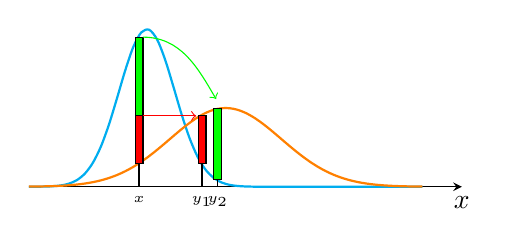
\begin{tikzpicture}
        % draw the axis
        \draw[eaxis] (-1.5,0) -- (4,0) node[below] {$x$};
        % draw the function (piecewise)
        \draw[elegant,domain=-1.5:3.5] plot(\x,{pow(e,-(\x)^2*4)*2});
        \draw[elegant,orange,domain=-1.5:3.5] plot(\x,{pow(e,-(\x-1)^2)});
        
        \draw[fill=red] (-0.15,0.3) rectangle (-0.05,0.9) node [anchor=east] (block1) {};
        \draw[fill=green] (-0.15,0.9) rectangle (-0.05,1.9) node [anchor=east] (block2) {};
        \draw[fill=red] (0.65,0.3) rectangle (0.75,0.9) node (block3) {};
        \draw[fill=green] (0.85,0.09) rectangle (0.95,0.99) node (block4) {};
        
        \draw (-0.1,0.3) -- (-0.1,0) node [anchor=north] {\tiny$x$};
        \draw (0.7,0.3) -- (0.7,0) node [anchor=north] {\tiny$y_1$};
        \draw (0.9,0.1) -- (0.9,0) node [anchor=north] {\tiny$y_2$};
        
        \draw[red,->] (block1) -- (block3);
        \draw[green,->] (block2) to[out=0, in=120] (block4);
    \end{tikzpicture}
    }
\end{frame}

\begin{frame}
    \frametitle{Wasserstein Distance}
    \resizebox{\textwidth}{!}{
    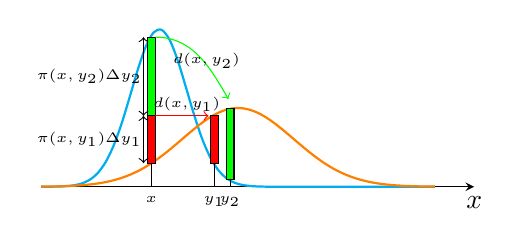
\begin{tikzpicture}
        % draw the axis
        \draw[eaxis] (-1.5,0) -- (4,0) node[below] {$x$};
        % draw the function (piecewise)
        \draw[elegant,domain=-1.5:3.5] plot(\x,{pow(e,-(\x)^2*4)*2});
        \draw[elegant,orange,domain=-1.5:3.5] plot(\x,{pow(e,-(\x-1)^2)});
        
        \draw[fill=red] (-0.15,0.3) rectangle (-0.05,0.9) node [anchor=east] (block1) {};
        \draw[<->] (-0.2,0.3) -- (-0.2,0.9);
        \node [anchor=east] at (-0.1,0.6) {\tiny$\pi(x,y_1)\Delta y_1$};
        \draw[fill=green] (-0.15,0.9) rectangle (-0.05,1.9) node [anchor=east] (block2) {};
        \draw[<->] (-0.2,0.9) -- (-0.2,1.9);
        \node [anchor=east] at (-0.1,1.4) {\tiny$\pi(x,y_2)\Delta y_2$};
        \draw[fill=red] (0.65,0.3) rectangle (0.75,0.9) node (block3) {};
        \draw[fill=green] (0.85,0.09) rectangle (0.95,0.99) node (block4) {};
        
        \draw (-0.1,0.3) -- (-0.1,0) node [anchor=north] {\tiny$x$};
        \draw (0.7,0.3) -- (0.7,0) node [anchor=north] {\tiny$y_1$};
        \draw (0.9,0.1) -- (0.9,0) node [anchor=north] {\tiny$y_2$};
        
        \draw[red,->] (block1) -- (block3);
        \node at (0.35,1.05)  {\tiny$d(x,y_1)$};
        \draw[green,->] (block2) to[out=0, in=120] (block4);
        \node at (0.6,1.6)  {\tiny$d(x,y_2)$};
    \end{tikzpicture}
    }
\pause
\begin{equation*}
    \begin{aligned}
        &\pi(x,y_1)\Delta y_1 + \pi(x,y_1)\Delta y_2 = \mu(x) - \nu(x) \\
        &\Delta W=\pi(x,y_1)\Delta x\Delta y_1 d(x,y_1) + \pi(x,y_2)\Delta x\Delta y_2 d(x,y_2) \\
    \end{aligned}
\end{equation*}
\pause
\begin{equation*}
    \begin{aligned}
    \therefore &\int \pi(x,y)\mathrm{d}y = \mu(x),\ \ \ \ \int \pi(x,y)\mathrm{d}x = \nu(y) \\
        &W(\mu(x),\nu(x))|_{\pi=\pi(x,y)} = \iint \pi(x,y)d(x,y)\mathrm{d}x\mathrm{d}y = \int d(x,y)\mathrm{d}\pi(x,y)\\
    \end{aligned}
\end{equation*}
\end{frame}
\begin{frame}
    \frametitle{Wasserstein Distance}
    \resizebox{\textwidth}{!}{
    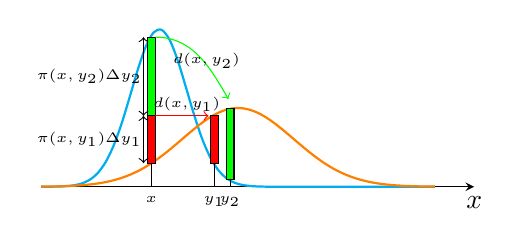
\begin{tikzpicture}
        % draw the axis
        \draw[eaxis] (-1.5,0) -- (4,0) node[below] {$x$};
        % draw the function (piecewise)
        \draw[elegant,domain=-1.5:3.5] plot(\x,{pow(e,-(\x)^2*4)*2});
        \draw[elegant,orange,domain=-1.5:3.5] plot(\x,{pow(e,-(\x-1)^2)});
        
        \draw[fill=red] (-0.15,0.3) rectangle (-0.05,0.9) node [anchor=east] (block1) {};
        \draw[<->] (-0.2,0.3) -- (-0.2,0.9);
        \node [anchor=east] at (-0.1,0.6) {\tiny$\pi(x,y_1)\Delta y_1$};
        \draw[fill=green] (-0.15,0.9) rectangle (-0.05,1.9) node [anchor=east] (block2) {};
        \draw[<->] (-0.2,0.9) -- (-0.2,1.9);
        \node [anchor=east] at (-0.1,1.4) {\tiny$\pi(x,y_2)\Delta y_2$};
        \draw[fill=red] (0.65,0.3) rectangle (0.75,0.9) node (block3) {};
        \draw[fill=green] (0.85,0.09) rectangle (0.95,0.99) node (block4) {};
        
        \draw (-0.1,0.3) -- (-0.1,0) node [anchor=north] {\tiny$x$};
        \draw (0.7,0.3) -- (0.7,0) node [anchor=north] {\tiny$y_1$};
        \draw (0.9,0.1) -- (0.9,0) node [anchor=north] {\tiny$y_2$};
        
        \draw[red,->] (block1) -- (block3);
        \node at (0.35,1.05)  {\tiny$d(x,y_1)$};
        \draw[green,->] (block2) to[out=0, in=120] (block4);
        \node at (0.6,1.6)  {\tiny$d(x,y_2)$};
    \end{tikzpicture}
    }
    Choosing the best transportaion $\pi(x,y) \in \Pi(\mu,\nu)$:
\begin{equation*}
    \begin{aligned}
        \mathrm{Wasserstein}(\mu(x),\nu(x)) &= \inf_{\pi \in \Pi(\mu,\nu)} W(\mu(x),\nu(x))|_{\pi=\pi(x,y)} \\
        &=\inf_{\pi \in \Pi(\mu,\nu)}\int d(x,y)\mathrm{d}\pi(x,y)\\
    \end{aligned}
\end{equation*}
\end{frame}   
% \end{document}
%         % 建立相对坐标系
%         % \draw[help lines,xstep=.1,ystep=.1] (-1.5,0) grid (pi,2);